% Chapter 1

\chapter{Machine learning} % Main chapter title

\label{Chapter2} % Change X to a consecutive number; for referencing this chapter elsewhere, use \ref{ChapterX}

\section{What is machine learning}
Machine learning is a subfield from Computer Science. It is a type of Artificial Intelligence which allow programs to learn without being explicitly programmed. \cite{coursera} \\
\\
There are two classes of machine learning algorithms. There is \textbf{supervised} learning and \textbf{unsupervised} learning. Supervised learning is trained using labeled data. Labeled data is data which consists of input data and the corresponding output data. Unsupervised learning uses unlabeled data. The data used to train machine learning algorithms is called a \textbf{training set}.\\
\\
A \textbf{training sample} is a data point in an available training set that is used in a predictive modeling task. For example, if machine learning is applied to spam filtering, the training set is a collection of emails, some of which are spam emails. A training sample would be a single email. For example, if we are interested in classifying emails, one email in our dataset would be one training sample. Alternative names are a training example or training instance. \\
\\
Machine learning is applied for predictive modeling. In predictive modeling, a particular process is modeled. Using a training set, the model tries to learn or approximate a particular function that, for example, let's us distinguish spam from non-spam email. This function is called the target function. To model the process, one or more \textbf{features} are extracted from the process. A feature is an individual property of a process. In the example of mails, a feature could be the textbody, or it could be the sender of the email.\\\\
This chapter gives an introduction to the mathematical background of machine learning. It starts with supervised learning, more particularly lineair and logistic regression. Lineair and logistic regression are used to explain the mathematical background and give an explanation of how the algorithms can be used. An explanation of how neural networks work is given. Finally, some notes about how it was decided to use a particular set of algorithms for intrusion detection systems.
\section{Lineair Regression}
Lineair regression is an statistical approach to model the relationship between an "output" value $y$ and one or more "input" values $X$. It belongs to the category of supervised learning. An example of this can be seen in Figure~\ref{fig:regression}. The black dots represent the data to be modeled. The blue line is the model. This example only has one "input" value, this specific case of regression is called simple linear regression. \cite{scikit-regression}

\subsection{Hypothesis}
Machine learning relies heavily on a hypothesis. This is a function that transform a given input to the machine learning algorithm into the required output. It is a function that tries to model the the target function. When only one feature is considered, a hypothesis is a function of the form: 
\begin{align}
H_0(x) = \theta_0 + \theta_1 * x
\end{align}
For example, we could use the grades of high school students to predict their chance of success at university. $x$ represents the grades (on a scale from 0 to 10) for students and $y$ is the chance of success. Given is input data (the black points) and from that data a hypothesis (the blue line) is constructed.

\begin{figure}[H]
\centering
\begin{tikzpicture}
  \begin{axis}[ 
    xlabel=$x$,
    ylabel={$y$},
    xmin = 0,
	xmax = 6,
  ] 
    \addplot {15 + 4 * x}; 
    \addplot[only marks] coordinates {
		(0, 15)
		(1, 21)
		(2, 27)
		(3, 32)
		(4, 35)
		(5, 28)
		(4, 27)
	};
  \end{axis}
\end{tikzpicture}
\caption{Lineair Regression} \label{fig:regression}
\end{figure}

\subsection{Multiple feature hypothesis}
\noindent The hypothesis function can be generalised for $N$ properties. It generally has the form:
\begin{align}
H_0(x) = \theta_0x_0 + \theta_1x_1 + ... + \theta_nx_n
\end{align}
$x_0$ always has the value 1. The $\theta$ values and the $x$ values can be represented using vectors:
\begin{align}
\theta = [\theta_0, \theta_1, ..., \theta_n]^T
X = [1, x_1, ... ,x_n]^T
\end{align}
Now the hypothesis function can be written as:
\begin{align}
H_0(x) = \theta^TX
\end{align}
When data follows a polynomial model, you could manipulate the feature so that the hypothesis forms a polynomial function, for example:
\begin{align}
H_0(x) = \theta_0 + \theta_1 * x + \theta_2 * \sqrt{x}
\end{align}
\subsection{Cost function}
In order to construct a good hypothesis function, good values of $\theta$ have to be found. This can be seen as a minimization problem. The difference between any output $y$ and $H_0(x)$ has to be minimized. More concretely, the squared difference has to be minimized. This is the MSE, "Minimum Squared Error" function or also called the cost function. The notation $x^{(i)}$ and $y^{(i)}$ is to denote the $i$th training sample. With dataset size $m$, the MSE is:
\begin{align}
J(\theta) = \dfrac{\sum\limits_{i=1}^m(H_0(x^{(i)}) - y^{(i)})^2}{2m}
\end{align}

\subsection{Gradient descent}
To solve the minimization problem, the first step is to start with $\theta$ and keep changing the values to minimize $J(\theta)$, this is an iterative approach.  Gradient descent is such an algorithm that can be used to find a solution to the minimization problem. Gradient descent is an algorithm that uses the gradient or derivative of a function to find a local minimum of that function. \\
\\
 \begin{figure}[H]
\centering
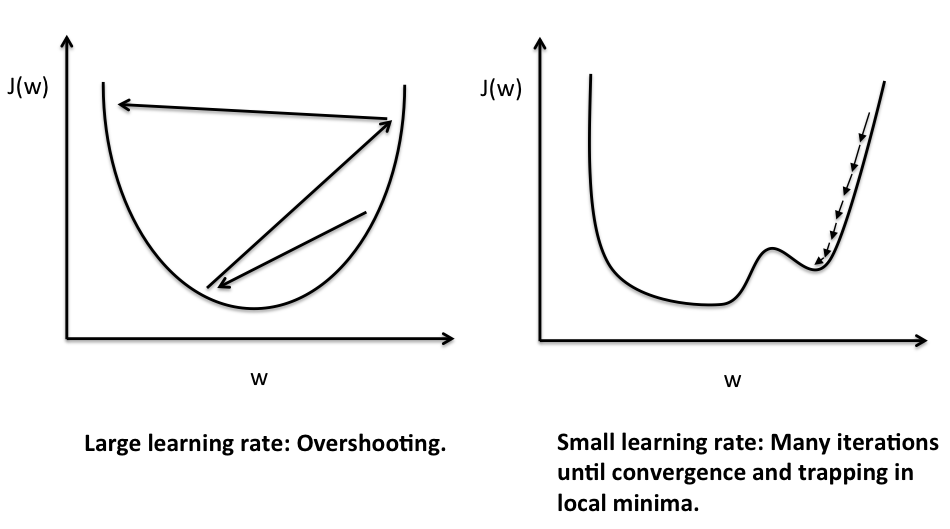
\includegraphics[width=1\textwidth]{Figures/gradient}
\decoRule
\caption[Gradient descent]{Iterations of gradient descent.}
\label{fig:gradient}
\end{figure}
\noindent A gradient descent algorithm does this using the following algorithm with a simultanious update for all values of $\theta$:
\begin{lstlisting}
            repeat until convergence {
 \end{lstlisting}
\begin{align}
    \theta_j = \theta_j - \alpha\dfrac{\partial}{\partial \theta_j}J(\theta)
\end{align}
\begin{lstlisting}
            }
 \end{lstlisting}
\begin{align}
\dfrac{\partial}{\partial \theta_j}J(\theta) =  \dfrac{\sum\limits_{i=1}^m(H_0(x^{(i)}) - y^{(i)}) * x_j^{(i)}}{m}
 \end{align}
 $\alpha$ is the learning rate of the gradient descent. The value of $\alpha$ describes how fast the gradient descent algorithm approaches the local mimimum. If $\alpha$ is too small, the gradient descent can be very slow. In the other case, if $\alpha$ is too large, the gradient descent can overshoot the local mimimum as seen in Figure~\ref{fig:gradient}. It may fail to converge and could even diverge. \\
 \\
The value of $\alpha$ does not need to change during the gradient descent, since the closer the gradient descent gets to the local mimimum, the smaller the derivative becomes, and smaller steps will be taken. If $\theta_j$ is already a local minimum, the derivative is $0$ and the gradient descent will not change the value of $\theta_j$.

\subsection{Feature scaling}
The main idea behind feature scaling is to make sure that the different features are on a different scale. The reason behind this is to optimize the gradient descent algorithm. When the scale is very different, the gradient descent will not alter $\theta_j$ much after each step. The range that should approximately be used is $-1 < x < 1$. \\
\\
Mean normalization could be used. This replaces each $x_i$ with $\dfrac{x_i - \mu_i}{s_i}$, where $\mu_i$ is the average value of all $x_i$ values and $s_i$ is the standard deviation.

\subsection{Normal equation}
For lineair regression, there is another method that could be used in place of gradient descent, a normal equation. This is a method to solve for $\theta$ analytically. But this method becomes slow when there are a lot of features. $X$ is a $m x n$ matrix constructed by putting all training samples (vectors of features) together. 
 \begin{gather}
 \dfrac{\partial}{\partial \theta_j}J(\theta) =  \dfrac{\sum\limits_{i=1}^m(H_0(x^{(i)}) - y^{(i)}) * x_j^{(i)}}{m} = 0\\
  \theta =  (X^TX)^{-1}X^Ty
  \end{gather}
But what happens when $(X^TX)$ is non-invertible, or singular. This means there are redundant features or more features than training samples. There are mathematical models, such as pseudo-inverse to still compute a correct result. There are still other methods that could replace gradient descent, such as conjugate gradient, BFGS and L-BFGS.

\section{Classification with logistic regression}
In a classification model, the machine learning algorithm tries to sort data into different classes. The simplest version is binary classification. For example, is the IP flow malicious or not. In lineair regression, the hypothesis can output values other than the classes that exist. However there is a method, logistic regression, which constrains the hypothesis to the available classes.

\subsection{Logistic regression}
Logistic regresion uses the Sigmoid or logistic function:
\begin{align}
g(z) =  \dfrac{1}{1 + e^{-z}}
\end{align}
\begin{figure}[H]
\centering
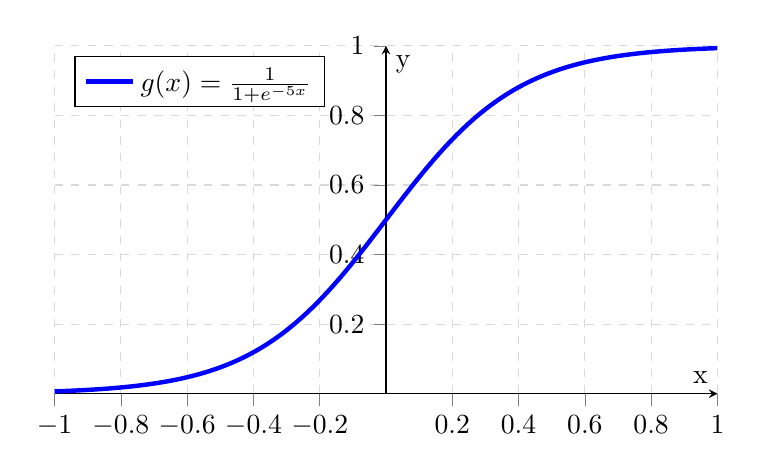
\begin{tikzpicture}
    \begin{axis}[
    	legend pos=north west,
        axis x line=middle,
        axis y line=middle,
        grid = major,
        width=10cm,
        height=6cm,
        grid style={dashed, gray!30},
        xmin=-1,     % start the diagram at this x-coordinate
        xmax= 1,    % end   the diagram at this x-coordinate
        ymin= 0,     % start the diagram at this y-coordinate
        ymax= 1,   % end   the diagram at this y-coordinate
        %axis background/.style={fill=white},
        xlabel=x,
        ylabel=y,
        tick align=outside,
        enlargelimits=false]
      % plot the stirling-formulae
      \addplot[domain=-1:1, blue, ultra thick,samples=500] {1/(1+exp(-5*x))};
      \addlegendentry{$g(x)=\frac{1}{1+e^{-5x}}$}
    \end{axis}
\end{tikzpicture}
\caption{Sigmoid function} \label{fig:logregression}
\end{figure}
\noindent Using this function, the hypothesis can be written as:
\begin{align}
H_0(x) = g(\theta^TX) = \dfrac{1}{1 + e^{\theta^TX}}
\end{align}
Ths hypothesis gives a probability. The decision boundary is $0.5$.
\subsection{Cost function}
The cost function from lineair regression cannot simply be applied to logistic regression. This cost function with the hypothesis of logistic regression is a non-convex function, a function with a lot of local minimums. A different cost function should be used:
\begin{gather}
J(\theta) = \dfrac{\sum\limits_{i=1}^m(Cost(H_\theta(x^{(i)}), y^{(i)}))}{m}\\
  Cost(H_\theta(x^{(i)}), y^{(i)}) =	\begin{cases}
        	 									     - log(H_\theta(x^{(i)})), & \text{if } y^{(i)} = 1\\
        									        - log(1 - H_\theta(x^{(i)})), & \text{if } y^{(i)} = 0\\
            									\end{cases}
\end{gather}
Gradient descent for logistic regression is exactly the same as for lineair regression except with a different hypothesis.

\subsection{Multi-class classification}
The above hypothesis and cost function are for binary classification. To compute multi-class classification, the One-vs-all algorithm could be used. This algortihm splits the multiples classes into two groups. One group contains one class, the other group contains all other classes. Using these two new groups, the algorithms for binary classification can be used. In other words, for each class $i$ a different logistic regression classifier $H_\theta(x)$ is trained to predict the probability that $y = 1$. On an input x, the most probable class is chosen.

\section{Overfitting}
When the data is not modeled correctly and the model is too precise for the training data, a problem called overfitting occurs. Models that are overfitted have high variance, there are too many possible hypothesis. In other words, if there are too many features, the hypothesis may fit the training set very well but fails too correctly predict new examples. In a similar way, underfitting may occur.
\begin{figure}[H]
\centering
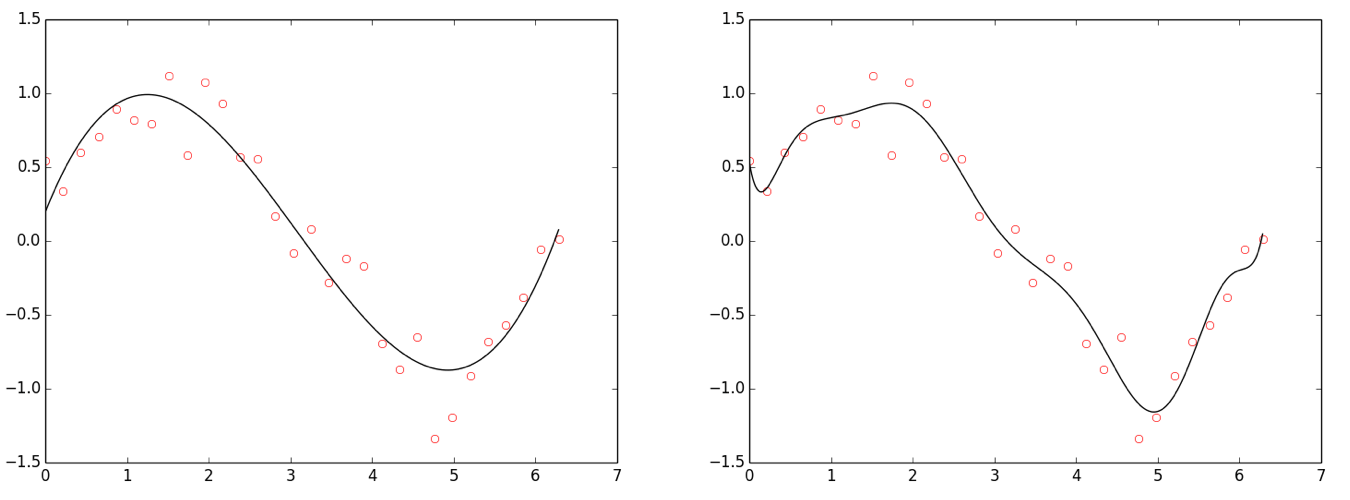
\includegraphics[width=1.2\textwidth]{Figures/overfit}
\decoRule
\caption[Overfitting]{The points are generated by a sin function with Gaussian noise. Left: good fit (polynomial of degree 3), Right: overfit (polynomial of degree 10).}
\label{fig:overfitting}
\end{figure}
\noindent There are methods to avoid overfitting. It is possible to reduce the amount of features.  This can be done manually or done by using a model selection algorithm. An other option is regularisation. This method keeps all features but manages the values of the parameters of $\theta$.  Regularisation works well when there are a lot of features that are all contribute to be able to predict $y$.

\subsection{Regularisation}
In regularisation, the parameters are being limited so that they are in scale with eachother. They should also be small. Bigger values for $\theta$, makes the hypothesis more prone to overfitting.  For lineair regression, this can be done in the cost function by redefining the cost function as:
\begin{align}
J(\theta) = \dfrac{\sum\limits_{i=1}^m(H_0(x^{(i)}) - y^{(i)})^2 + \lambda * \sum\limits_{j=1}^m(\theta_j^2)}{2m}
\end{align}
Only $\theta_1$ till $\theta_m$ should be regularised. $\lambda$ is called the regularisation parameter. \\

\noindent For lineair regression, the gradient descent is slightly different because of the modified cost function, the new cost function is:
\begin{lstlisting}
            repeat until convergence {
 \end{lstlisting}
\begin{align}
    \theta_j = \theta_j - \alpha * [  \dfrac{\sum\limits_{i=1}^m(H_0(x^{(i)}) - y^{(i)}) * x_j^{(i)}}{m} +  \dfrac{\lambda}{m} * \theta_j]
    \end{align}
\begin{lstlisting}
            }
 \end{lstlisting}
 \noindent For the normal equation a similar modification occurs. 
For logistic regression, the modification is analogous to the modification for lineair regression.

\section{Neural networks}
Neural networks are a usefull alternative to logistic regression if the amount of features becomes too large. The origin of neural networks are algorithms which try to mimic the brain. There is a hypothesis, the "one learning algorithm" hypothesis, that shows that the brain can learn very different things, such as sound, touch, etc. by using a single algorithm. \\\\
A neural network is created of neurons, which are called a logistic unit. Each neuron receives input wires, and has an output wire, which computes a value using the sigmoid (logistic) hypothesis, the activation function. A neural network is a group of "neurons" that are connected together. This can be grouped into a layered approach as seen in Figure~\ref{fig:neuralnetwork}. The first layer is called the input layer, the final layer is called the output layer which outputs a $H_\theta(x)$ which is class. All layers inbetween these layers are called hidden layers.
\begin{figure}[H]
\centering
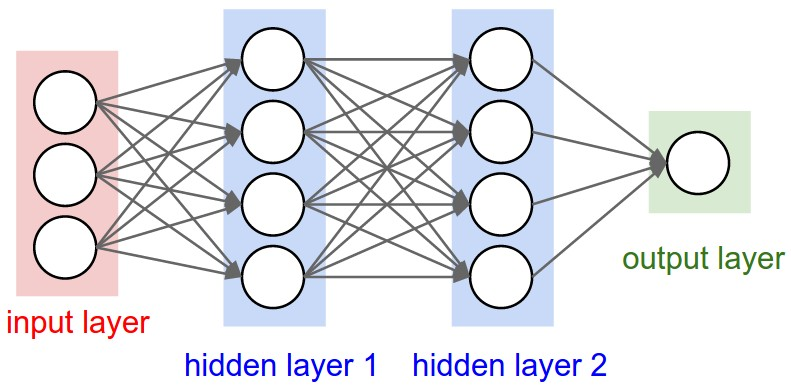
\includegraphics[width=1\textwidth]{Figures/neuralnet}
\decoRule
\caption[Neural network]{A neural network showing the different layers.}
\label{fig:neuralnetwork}
\end{figure}
\noindent Each logistic unit is denoted by $a_i^j$. $j$ is the layer and $i$ is the position in that layer. $\theta^j$ is a matrix of weights or parameters controlling function mapping from layer $j$ to layer $j+1$. $s_l$ is the number of units within a layer. The number of layers is denoted by $L$.\\\\The neural network works similar to logistic regression, except that it performs logistic regression from layer to layer. The parameters $\theta_j$ required are learned by itself. The architecture of a neural network refers to the way the units are connected to eachother. Neural networks can be used for multi-class classification. Hereby there are mutliple units in the output layer and each unit represents a different class. $K$ will denote the amount of output units.
\begin{figure}[H]
\centering
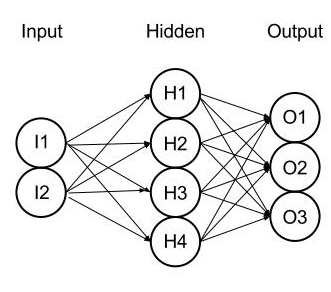
\includegraphics[width=0.7\textwidth]{Figures/neuralnetmulti}
\decoRule
\caption[Neural network with multi-class classification]{A neural network capable of multi-class classification.}
\label{fig:neuralnetworkmult}
\end{figure}
\noindent Data flows using the principle of forward propagation. The data passes through the first layers, move to the second layers and so on, until it arrives at the final layer. Mathematically this can be described as: 
\begin{align*}
a^{(1)} = x\\
z^{(2)} = \theta^{(1)}*a^{(1)}\\
a^{(1)} = g(z^{(2)})
\end{align*}
\subsection{Cost function and backpropagation}
The cost function for neural networks is a generalisation of the cost function for logistic regression. The cost function accounts for the different layers, units and the number of output units. To minimize the cost function, the same methods such as gradient descent can be used. However, the problem is how to compute the partial derivative of the cost function. Using backpropagation, it is possible to compute this. \\\\
The resulting class is known in the final layer. From here, the algorithm can find the error. $\delta_j^l$ will be the symbol used for the error of node $j$ in layer $l$. For an example with 4 layers:
\begin{align}
\delta_j^{(4)} = a_j^{(4)} - y_j\\
\delta^{(3)} = (\theta^{(3)})^T\delta^{(4)} * g'(z^{(3)})
\end{align}
The algorithm starts by setting a parameter $\Delta_{ij}^{(l)}$ to 0 for all $i$, $j$, $l$. Then, it iterates from $i=0$ to $m$, with $m$ the number of training samples. Each iteration, $a^{(1)}$ is set to $x^{(i)}$. Forward propagation is computed for $a^{(l)}$ for all $l = 2,3,..., L$. Using $y^{(i)}$, $\delta^{(L)}$ can be computed. Then the different $\delta^{(L-1)}$ to $\delta^{(2)}$ are computed. Finally, $\Delta_{ij}^{(l)}$ is incremented by $a_j^{(l)}\delta^{(l+2)}$ for each $l$. After the iteration is done, the final value for the partial derivative can be calculated: $\dfrac{\partial}{\partial \theta_ij^{(l)}} J(\theta)$. This can be done by dividing $\Delta_{ij}^{(l)}$ by the amount of training samples and adding $\lambda\theta_ij^{(i)}$. 
\subsection{Using a neural network}
A neural network should have as many input units as the dimension of features. The number of output units is equal to the number of classes. Default, there should be either 1 hidden layer or if there are more, all layers should have the same number of hidden units. The neural network should be trained by first assigning random weights to the values of $\theta$. Afterwards, forward propagation should be used to get $H_\theta(x^{(i)}$. Next the cost function should be computed. Backwards propagation is used to compute the partial derivatives. The result of backwards propagation can be checked by numerical methods to compute the gradient. Finally gradient descent or other advanced optimization methods with backpropagation should be used to try to minimize the cost function as a function to the parameters $\theta$.
\section{Support Vector Machines}
Support vector machines or SVMs is a supervised learning algorithm which offers an alternative view on logistic regression. Support vector machines try to find a model which devides the 2 classes exactly with the same amount of margin on either side as shown in Figure~\ref{fig:svm}. Samples on the margin are called the support vectors.
\begin{figure}[H]
\centering
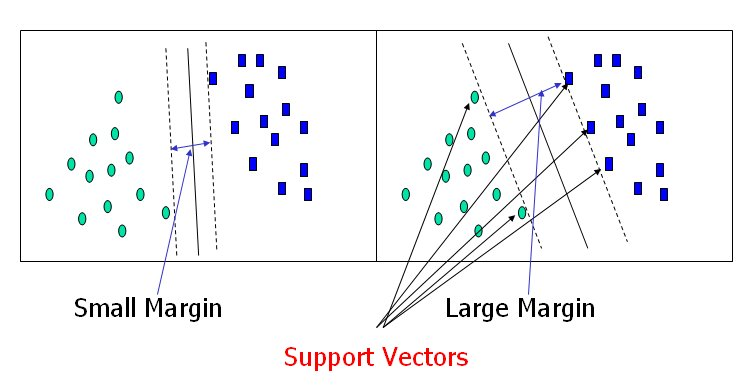
\includegraphics[width=\textwidth]{Figures/svm}
\decoRule
\caption[Support Vector Machines]{Support vector machines with their support vectors.}
\label{fig:svm}
\end{figure}
\noindent In order to adapt Support Vector Machines to be able to fit non-lineair classifiers, some adjustments need to be done. This can be done with kernels. A kernel is a similarity function. The function compares two inputs and computes their similarity. Normally features are extracted from data and then fed into a machine learning algorithm. Kernels offer an alternative. The kernel should be a function to compare input data. The kernel, along with labeled data is then used to construct features. Using no kernel is called a lineair kernel. The basic type of kernel algorithms are called Gaussian kernels. The formula for Gaussian kernels is:
\begin{align}
K(x,y) = \exp{(\dfrac{-||x-y||^2}{2\sigma^2})}
\end{align}

\section{K-Nearest Neighbors}
The K-Nearest Neighbors or KNN algorithm is an algorithm which computes the classification by looking at the classes of the K-Nearest neighbors of the inputted data. The K-Nearest Neighbors is a Instance-based algorithm. \cite{mlcat} The chosen class is the class most common among its K-Nearest neighbors, this can be seen in Figure~\ref{fig:knn}. K is typically a small number. When K is equal to 1, the assigned class is the same as the class of the closest sample. \\\\
When training the algorithm, the input data and classes are stored. There are mutliple method to compute the distance between data. Euclidean distance can be used for continous data. For discrete variables another metric can be used, such as the overlap metric or Hamming distance.\\\\
A major drawback of the KNN algorithm is the weakness to skewed data. Since the class is chosen based on the most popular nearest class, these popular classes may dominate the prediction. This can be overcome by taking the distance between the input data and the neighbors into account. \\\\
Because KNN looks at the nearest neighbors, it effectively is a clustering algorithms. This is useful to know when trying to evaluate which algorithm should be used for a certain problem.
\begin{figure}[H]
\centering
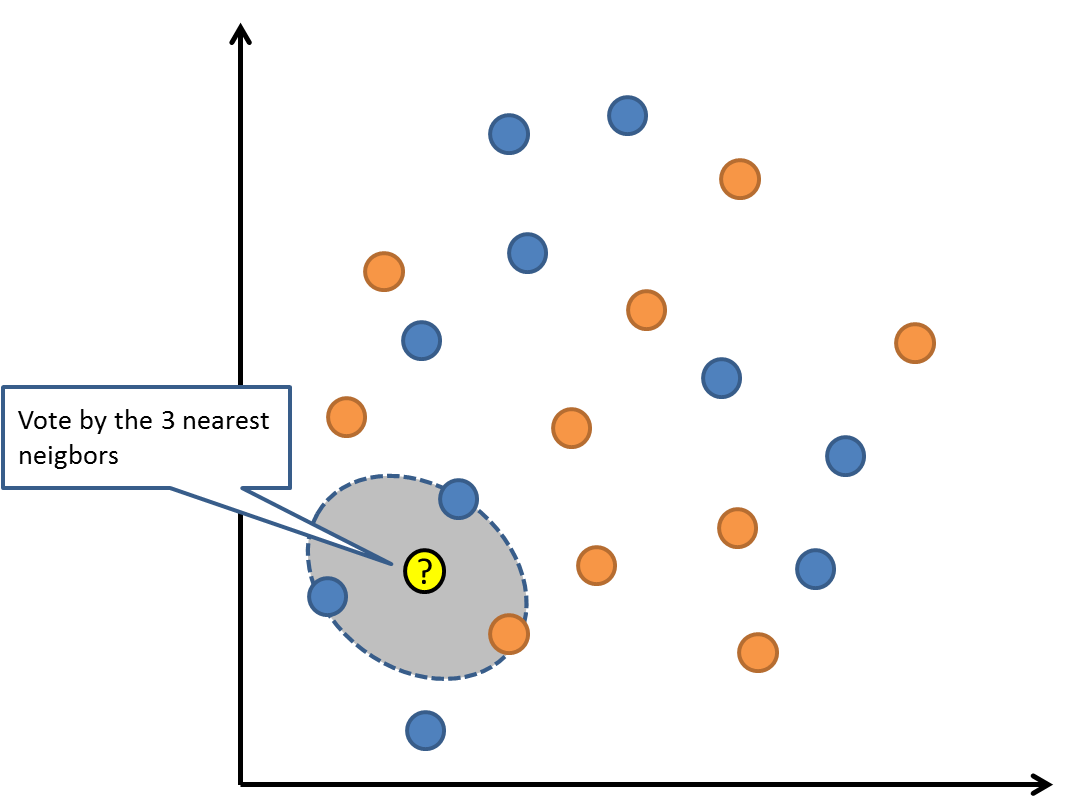
\includegraphics[width=0.8\textwidth]{Figures/knn}
\decoRule
\caption[K-Nearest Neighbors]{K-Nearest Neighbors.}
\label{fig:knn}
\end{figure}

\section{Clustering}
Clustering a machine learning concept using unsupervised learning. Unsupervised learning does not have labels with the training set. An unsupervised machine learning algorithm tries to find structure within the given training set. Clustering is the first type of unsupervised learning. It tries to cluster the training samples into different clusters.

\subsection{K-means Algorithm}
The K-means algorithm is a simple clustering algorithm. K is the number of clusters that is going to be used. The algorithm first randomly places the K clusters in the space (from the training set). This can be done by randomly chosing K training samples. Then it repeats the following steps until the cluster centers remain stationary. it iterates over all training samples, and assigns them to the closest cluster. Next the cluster centers are moved to the center of the total cluster. \\\\
The cluster centroids will be addressed using the symbol $\mu$ with $\mu_k$ the cluster centroid of cluster k. $c^{(i)}$ is the index of the cluster to which training sample  $x^{(i)}$ has been assigned. $\mu_{c^{(i)}}$ is the cluster centroid to which training sample $x^{(i)}$ has been assigned. The cost function can be described as:
\begin{align}
J(c, \mu) = \dfrac{1}{m} \sum\limits_{i=1}^m(|| x^{(i)} - \mu^{(i)}||^2
\end{align}
With the randomly chosing K clusters, it could be that the K-means algorithm only find small local cluster and give suboptimal results. This can be fixed by running the randomly chosing and K-means a number of times and after each iteration check the value of the cost function to find the most efficient clusters. The same method could be used to determine the correct number of clusters. However, manually determining the number of clusters could be more efficient.

\section{Dimensionality reduction}
Dimensionality reduction is the process of reducing the amount of features used in machine learning algorithms. This can be used to increase the accuracy and the performace of machine learning algorithms. One form is to do data compression. For example, transform 3D data into 2D data and eliminating a feature or dimension. It can also be used to reduce dimensions to be able to efficiently visualise data.

\subsection{Principle Component Analysis}
Principle Component Analysis is a way to do dimensionality reduction. The algorithm is formed as a minimalisation problem. When given N-dimensional data and N-1 dimensional data is prefered. The algorithm tries to find the correct N-1 dimensional value so that the projection is the closest to the original data. \\\\
Before this algorithm should be run, the features of the data should be scaled, so all features are on a similar scale. This can be done by using mean normalization. In order to reduce the dimension from $n$ to $k$ the covariance matrix should be computed:
\begin{align}
\Sigma = \dfrac{1}{m}\sum\limits_{i=1}^n((x^{(i)}) (x^{(i)})^T)
\end{align}
From this matrix, the eigenvectors need to be computed using singular value decomposition. From these values, only the first $k$ values are going to be used and be multiplied with the training data.\\\\
PCA can be used to speed up the time it takes for other learning algorithms to learn. By using PCA, the amount of features or the amount of training samples is reduced which reduces the running time of the training, but the compressed data still retains the same information as the uncompressed data.

\section{Anomaly detection}
Anomaly detection is also a form of unsupervised learning. The algorithm learns what normal behaviour looks like through the training set and then tries to predict if a given input data belongs to the normal behaviour or is abnormal for any reason.
\begin{figure}[H]
\centering
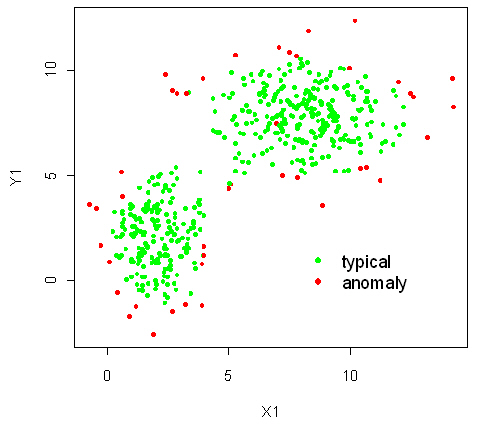
\includegraphics[width=0.8\textwidth]{Figures/anomaly}
\decoRule
\caption[Anomaly detection]{Anomaly detection.}
\label{fig:anomalydetection}
\end{figure}
\noindent Anomaly detection algorithms make heavy use of (Gaussian) Normal distribution:
\begin{align}
x \sim N(\mu, \sigma^2)
\end{align}
Hereby is $\mu$ the mean parameter and $\sigma$ is the standard deviation. Now the probability of $x$ being an anomaly can be calculated as:
\begin{align}
p(x) = \prod_{j=1}^n( \dfrac{1}{\sqrt{2\pi}\sigma_j} exp(- \dfrac{(x_j - \mu_j)^2}{2\sigma_j^2}) )
\end{align}

\section{Other algorithms}
There are also other, more specific and advanced categories of machine learning algorithms. There are decision tree algorithms, for example, Classification and Regression Tree (CART), Conditional Decision Trees, etc. There are Bayesian Algorithms which explicitly apply Bayes’ Theorem for problems such as classification and regression. These algorithms include Naive Bayes, Gaussian Naive Bayes, Multinomial Naive Bayes, etc. \cite{mlcat} \\\\
Association Rule Learning Algorithms are methods that extract rules that best explain observed relationships between variables in data. Apriori algorithm and Eclat algorithm are examples of such algorithms. Deep Learning Algorithms are a modern modification to Artificial Neural Networks that exploit abundant cheap computation. Deep learning networks are very deep and complex neural networks. Deep Boltzmann Machine (DBM), Deep Belief Networks (DBN) and Convolutional Neural Network (CNN) are examples of deap learning algorithms.  \cite{mlcat}\\\\
Ensemble Algorithms such as Bootstrapped Aggregation (Bagging) are models that combine multiple weaker models and try to combine the predictions made by these models. Yet there are still many more algorithms.  \cite{mlcat}\\\\
A lot of algorithms are specifically constructed for a specific sub-field of machine learning, for example computer vision, natural language processing, etc. Even within the categories of algorithms that were discussed, regression, regularization, instance-based, clustering, neural networks and dimensionality reduction, there are a lot of different variants. However, these are considered to be to advanced and outside the scope of this thesis. 

\section{Machine learning diagnostic}
Machine learning diagnostics are tests that can be run to get to know what is and isn't working with a machine learning algorithm. They also provide guidance as to how performance could be improved. 

\subsection{Evaluating the hypothesis}
The most obvious way to test whether the hypothesis is correct is by dividing the training set into two sets. The first set which should have approximatly 70\% of the samples of the original training set will be used to train the learning algorithm. The other set is used to check whether the output of the learning algorithm is correct. If the output isn't correct, a test error can be computed. These test errors can be used to compute global error value, which could be calculated by, for example, a mean squared error. This value can be used ito evaluate the hypothesis.

\subsection{Model selection algorithm}
To get back to the problem of overfitting, there is another method next to regularisation called model selection. Model selection uses the same principle as mentioned above except it divides the training set into three new sets. A new training set, a cross validation set and a test set. Different models can be tested and compared to eachother by comparing the cross validation error. It is considered good practice to use seperate sets for cross validation and testing.

\subsection{Diagnosing bias vs variance}
High variance means that there is an overfitting problem. High bias on the other hand, is the opposite problem. It means that the hypothesis does not fit the training set at all.
\begin{figure}[H]
\centering
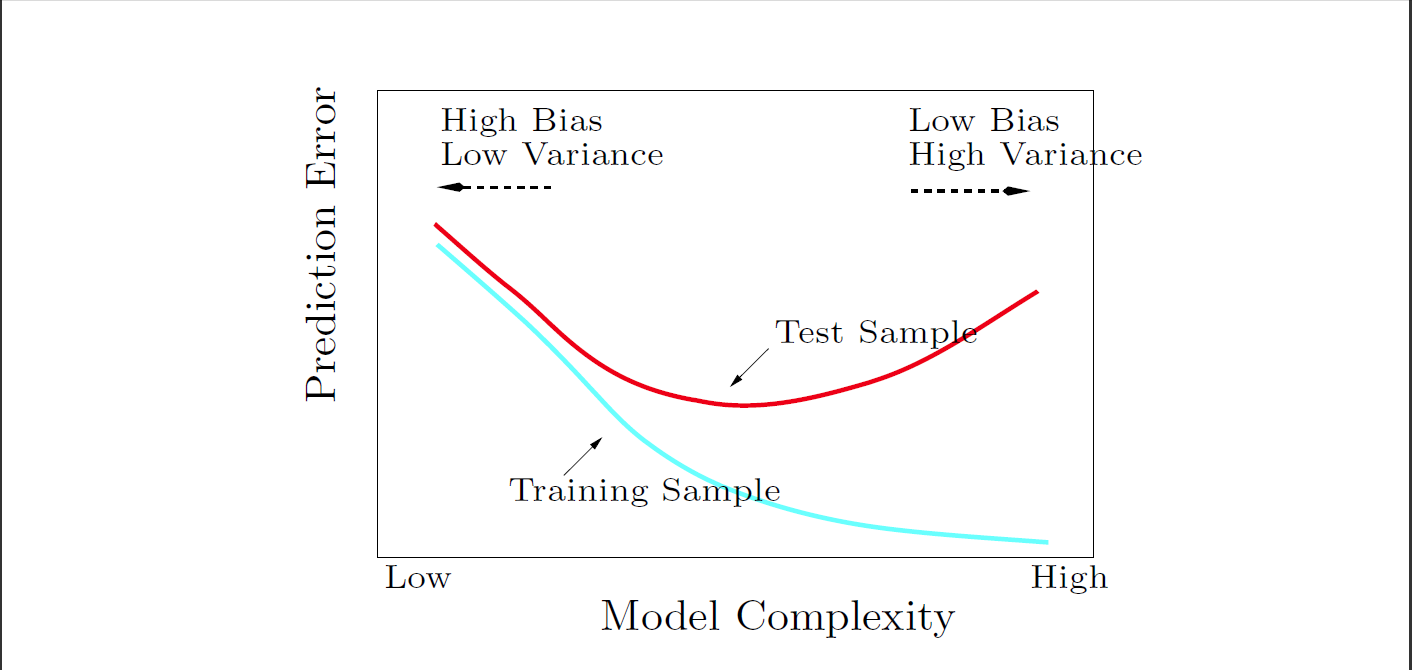
\includegraphics[width=\textwidth]{Figures/biasvariance}
\decoRule
\caption[High bias vs high variance]{The difference between high bias and high variance.}
\label{fig:biasvariance}
\end{figure}
\noindent With a low model complexity, there is a high error for the training set and a high error on the test set. This is a signal there is a underfitting problem or a bias problem. With a high complexity model, the training set error is very low, but the test set error is very high. This is a signal there is an overfitting problem or a variance problem. This can be seen in Figure~\ref{fig:biasvariance}. The complexity of the model can be adjusted by changing the amount of features that are being used. 

\subsection{Learning curves}
There is a relation between the amount of training samples and the training error. With more training data, the training error goes down. However, with high bias, it does not help to increase the amount of training samples.
\begin{figure}[H]
\centering
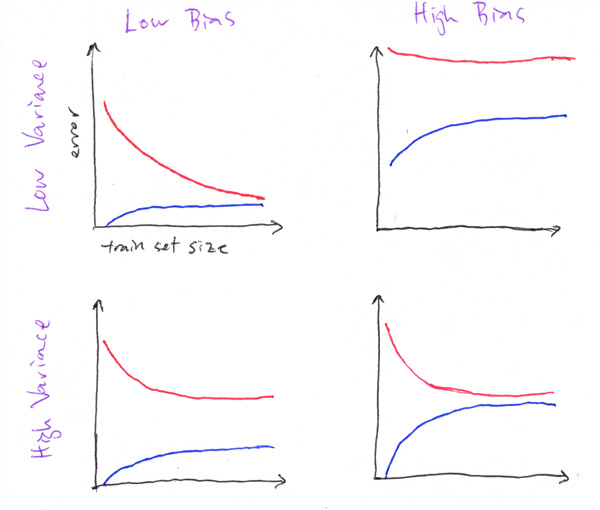
\includegraphics[width=0.8\textwidth]{Figures/bias_variance_chart}
\decoRule
\caption[Training samples comparison]{The effect of the amount of training samples on the accuracy.}
\label{fig:trainingsamples}
\end{figure}
\noindent In Figure~\ref{fig:trainingsamples} the general trend of training error and test (or true) error is shown. This figure shows the example for high bias and no matter how many training samples there are, the functions are already converged to the same error amount.\\\\
In contrary to high bias, high variance can be solved by using extra training samples. In that case there is a gap inbetween the true error line and the training error line and it is likely that they still converge to the same point. With a bigger training set, they converge more and more.

\section{Machine learning system design}
When trying to use machine learning for any purpose, such as intrusion detection systems. There are several considerations to be made. Another important step is the approach used to find the correct algorithm. 
The recommended approach is to start with a simple algorithm and test it with cross validation data. Afterwards, learning curves could be plotted to decide if more or less data, more or less features, ... are likely to help. Finally, error analysis can be done by maually examining the samples on which the algorithm made mistakes. This could help to spot any systematic trends in the type of samples on which the algorithm is making mistakes.\\\\
The error analysis mostly consists of manual work. The samples on which the algorithm is wrong need to be categorized based on which features could help it categorize correctly and on which class it belongs to. Calculating statistics, such as the accuracy of the algorithm can also help with error analysis. \\\\
Another issue to account for are skewed classes. Skewed classes are classes that are underrepresented in training data. For example, in binary classification, when trying to classify a flow as malicious or not, the training set might only provide $0.5$\% malicious data. Knowing this, having an accuracy of $99$\% does not seem that great.

\begin{figure}[H]
\centering
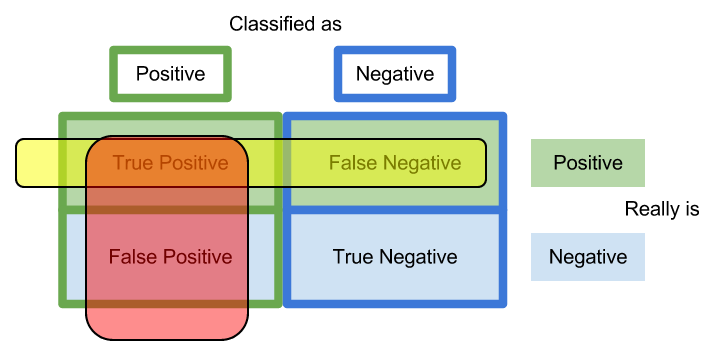
\includegraphics[width=1\textwidth]{Figures/precisionrecall}
\decoRule
\caption[Precision and recall]{Precision and recall.}
\label{fig:precisionrecall}
\end{figure}
\noindent A different metric is required to evaluate machine learning algorithms that are trained using skewed data. This metric is the precision and recall method. We classify a result as true positive, true negative, false positive and false negative. False positive and false negative respectively mean that the predicted value is falsely classified as positive and negative. These are the errors. True positive and true negative are correctly predicted values. Precision is defined as the fraction of predicted malicious flows that were actually malicious: 
$$\dfrac{true positive}{true positive + false positive}$$
Recall is defined as the fraction of predicted malicous flows and the actual amount of malicous flows: 
$$\dfrac{true positive}{true positive + false negative}$$
There is always a tradeoff to be made between precision and recall. As an effect of a higher precision, there will be a lower recall. Similarly, a higher recall means a lower precision.\\\\
Algorithms with a different precision and recall can be compared to eachother. This can be done using an F-score: 
$$2 \dfrac{PR}{P+R}$$
\noindent For Table~\ref{tab:precrecal}, this means that Algorithm 1 is the most effective. In contrast, using for example the average of both precision and recall would make Algorithm 3 the most effective.
\begin{table}[H]
\caption{Example of precision and recall of certain algorithms.}
\label{tab:precrecal}
\centering
\begin{tabular}{| l | c  r|}
\toprule
\tabhead{} & \tabhead{Precision (P)} & \tabhead{Recall (R)}\\
\midrule
Algorithm 1 & 0.5 & 0.4\\
Algorithm 2 & 0.7 & 0.1\\
Algorithm 3 & 0.02 & 1.0\\
\bottomrule
\end{tabular}
\end{table}
\noindent The data that is being fed into a machine learning algorithm is also important to consider. Sometimes a lot of data can be useful. First, the assumption is made that the features are chosen correctly and sufficiently. Lots of data is useful when a machine learning algorithm is used with a lot of parameters such as a neural network with a lot of hidden units. This means that the algorithm has low bias. 

\subsection{Different Algorithms}
If the number of features is large relative to the number of training samples, then using a lineair kernel Support Vector Machine or logistic regression. A Gaussian kernel is preferred when there are more training samples than features, but the difference is rather small. Otherwise, new features should be added. Neural networks are almost always effective but they may be slower to train.\\\\
In problem of intrusion detection system, there are a small number of features and a large number of training samples. 